\documentclass{acm_proc_article-sp}
\usepackage{svg}
\usepackage{listings}
% \usepackage{ref}
\lstset{
    numberblanklines=false,
    language=make,
    tabsize=4,
    frame=single,
    keywordstyle=\color{red},
    identifierstyle= %plain identifiers for make
}
\begin{document}

\title{
Looking Back at the BEAST Attack
%\titlenote{(Does NOT produce the permission block, copyright information nor page numbering). For use with ACM\_PROC\_ARTICLE-SP.CLS. Supported by ACM.}
}
\numberofauthors{5}
\author{
\alignauthor
Yang Shichu\\
    \affaddr{Huazhong University of Science and Technology}\\
    \email{sigeryeung@gmail.com}
\alignauthor
Shu Yi\\
    \affaddr{Huazhong University of Science and Technology}\\
    \email{1907230957@qq.com}
\alignauthor
Su Haochen\\
    \affaddr{Sichuan University}\\
    \email{suhaochen163@163.com}
\and
\alignauthor
Li Yucong\\
    \affaddr{Shandong University}\\
    \email{lycbin@gamil.com}
\alignauthor
Liao Haicheng\\
    \affaddr{University of Electronic Science and Technology of China}\\
    \email{LiaoHaicheng25@163.com}
}
\date{27 July 2021}
\maketitle
\begin{abstract}
Transport Layer Security (TLS) is an protocol that provides communication
security over networks. However, there is a flaw in TLS 1.0 where the initial
vectors for block ciphers are predictable. The BEAST attack, with some
prerequisites and efforts, allows attackers in the middle to decrypt those
encrypted messages without knowing the key.
This paper will demonstrate the procedures of the BEAST attack, and propose
methods in simulation and vulnerability detection.
\end{abstract}

% A category with the (minimum) three required fields
% \category{H.4}{Information Systems Applications}{Miscellaneous}
%A category including the fourth, optional field follows...
% \category{D.2.8}{Software Engineering}{Metrics}[complexity measures, performance measures]

% \terms{}

\keywords{BEAST attack, TLS flaws, CBC exploits, vulnerability detection} % NOT required for Proceedings

\section{Introduction}
Transport Layer Security (TLS) has several versions. The specification for TLS
1.0 is RFC 2246\cite{rfc2246}.
In this paper we will show a flaw in one of the common modes of operation used in block ciphers
and how it allows for a specific kind of attack\cite{beast} on HTTPS.

%\end{document}  % This is where a 'short' article might terminate
\section{Background}
\subsection{A glance at TLS}

TLS is a protocol for safe data transferring that works between the transport layer
and the application layer. The cipher suites used in TLS often involve an asymmetric cipher
(e.g. RSA) for key exchanging and a symmetric block cipher (e.g. AES) for message encryption.
The protocol is widely used together with data transfer applications such as HTTP, FTP and SMTP.

\subsection{CBC in block ciphers}
Cipher Block Chaining (CBC) is one of the modes of operation used in block ciphers.
In order to reduce the time spent on generating random initialization vectors (IVs), CBC always takes
the previous encrypted ciphertext block and use it as the IV for the current plaintext block before the
block cipher encrypts, except for the first block as shown in \ref{fig:cbc-encryptor}.

Suppose that $P_1,P_2,\cdots P_n$ are the plaintext blocks, with a initialization vector $IV$, we have:

$$
\begin{aligned}
C_1&=E_k(P_1\oplus IV)\\
C_i&=E_k(P_{i}\oplus C_{i-1}) (i\geq 2)
\end{aligned}
$$

to obtain ciphertext blocks $C_1,C_2,\cdots,C_n$.

\begin{figure}[htb]
  \centering
  \includesvg[keepaspectratio, width=\linewidth]{./figures/cbc-encryptor.drawio.svg}
  \caption{CBC encryptor}
  \label{fig:cbc-encryptor}
\end{figure}

\section{The BEAST Attack}
\subsection{Predictable IV and Consequences}
As we mentioned in Section 2.2, a block cipher using CBC always takes its previous cipher block as
its next IV. This means that an attacker who has been eavesdropping the whole encrypted
conversation can infer all the IVs in the conversation except for the first one.
If the attacker has control over such an encryption machine (i.e. he has chosen plaintext privilege),
in an attempt to guess the plaintext of block $C_k$ with a guessed plaintext block $P_k'$,
assuming the encryption machine is about to encrypt the $i+1$th block,

he can pass
$$
\begin{aligned}
P_{i+1}&=P_k'\oplus C_i\oplus C_{k-1}
\end{aligned}
$$
to the machine. So that the ciphertext block would be
$$
\begin{aligned}
C_{i+1}&=E_k(P_k'\oplus C_i\oplus C_{k-1}\oplus C_i)=E_k(P_k'\oplus C_{k-1})
\end{aligned}
$$
Since the block cipher algorithm used in TLS is deterministic
(i.e. same plaintext encrypts to same ciphertext),

and $C_k = E_k(P_k\oplus C_{k-1})$,

If $C_{i+1} = C_k$, then
$$
\begin{aligned}
P_k\oplus C_{k-1}&= P_k'\oplus C_{k-1}\\
P_k&= P_k'
\end{aligned}
$$
The procedure shown above is actually a validation oracle which tells whether the attacker's guess
on $P_k$ is correct. In conclusion, an attacker with chosen plaintext privilege in this case can use
brute force to obtain the plaintext of any cipher block $C_k(k\geq 2)$.
\subsection{Chosen Boundary Attacks}
\subsubsection{Failure of chosen plaintext}
The chosen plaintext attack shown above requires that the attacker guesses the content of a whole
block every time. Although this effectively gets IVs from CBC mode out of the way, it is still not a
practical attack as the time required to decrypt a single block would be sufficiently long.
For Advanced Encryption Standard (AES), a commonly used block cipher,
the block size is 16 bytes\cite{aes} which means an attacker would have to guess up to $2^{128}$
blocks for one ciphertext block.
This is considered secure as AES is designed with a 128-bit security level\cite{seclv} and this
security level is unharmed. So for an attack to work, it needs to further reduce the number of guess
trials.
\subsubsection{The BEAST}
Recall that in Section 3.1 we mentioned an attacker with chosen plaintext privilege. Here we
will show that if such an attacker further gains chosen boundary privilege, he can decrypt a secret
string with far less trials than a simple brute force attack. The chosen boundary privilege means that
the attacker can force the victim to send cookie-bearing requests with arbitrary request paths to the
HTTPS server. If the attacker gains this privilege, he can carefully craft the request path so that
exactly 1 byte of the target string will be placed at the end of a plaintext block while the rest is at the
beginning of the next plaintext block. An example of such a request is shown in \ref{fig:req-example}.

\begin{figure}[htb]
    \centering
    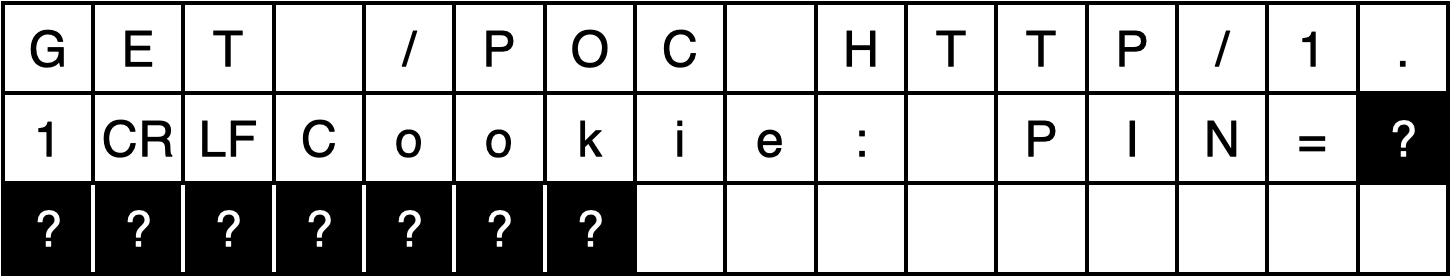
\includegraphics[keepaspectratio, width=\linewidth]{./figures/request-example.png}
    \caption{chosen boundary request example}
    \label{fig:req-example}
\end{figure}
In this case, 15 out of 16 bytes in the second plaintext block is
already known to the attacker. Now the attacker performs the same chosen plaintext attack
described in Section 3.1 except that he only has to guess 256 times to obtain the first byte of the
secret string.

After obtaining the first byte of the secret, the attacker reduces the length of the request path by 1
byte, so 2 bytes of the secret are now at the end of the plaintext block. As the first byte is already
compromised, the attacker can use the same technique above to obtain the second byte with only
256 guesses. Repeating the steps shown above, the attacker can eventually reveal the whole secret
string with chosen boundary requests as in \ref{fig:reveal} (showing only the block to guess).
\begin{figure}[htb]
    \centering
    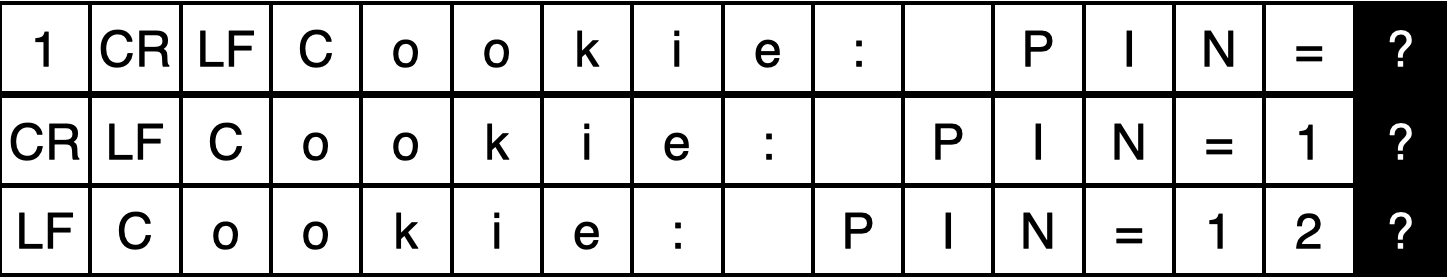
\includegraphics[keepaspectratio, width=\linewidth]{./figures/revealing.png}
    \caption{revealing the secret bytes 1 by 1}
    \label{fig:reveal}
\end{figure}

In this attack scenario, only $256\times16 = 2^{12}$ guesses are needed to decrypt an entire block 
of secret, effectively reducing the 128-bit security level in AES to only 12 bits. As this attack aims at
breaking certain ciphers used in Secure Sockets Layer (SSL) and TLS and requires chosen
boundary privilege which is often obtained by injecting malicious JavaScript into a webpage,
this kind of attack is therefore named Browser Exploit Against SSL/TLS (BEAST).

\section{Threat Model}
\subsection{Prerequisites for attackers}
In order to mount such an attack, the attacker must have these capabilities:
\begin{itemize}
    \item \textbf{Network Eavesdropping} The attacker must be able to capture the whole 
    encrypted conversation to know every IV in the process. This information is obtainable most
    of the time, yet certain protocols used at link layer (e.g. Wi-Fi with Pre-Shared Key, Virtual Private
    Networks) may prevent this.
    \item \textbf{Chosen Plaintext} The attacker can construct any known plaintext block and force the
    client to encrypt and send it via HTTPS. This allows for guessing the content of a ciphertext block.
    \item \textbf{Chosen Boundary} The attacker should be able to force the client to send arbitrary
    requests with cookie to the HTTPS server. By controlling the resource path, the attacker is able to
    place the secret cookie anywhere in a plaintext block.
\end{itemize}
\subsection{Server vulnerability}
The BEAST attack only works against TLS Version 1.0 and requires a block cipher working in CBC
mode. For the attacker to gain chosen plaintext privilege, the server must also host a WebSocket
service that allows sending arbitrary plaintext without any formatting. This is further addressed in
Section 6.1, where we discuss why BEAST attack fails in front of the latest security standards.

\section{Demonstration}
In this section, we show how we simulated a BEAST attack using raw socket over TLS.
Our simulation is based on the Docker virtualization platform, and we use the TLSAutomaton API
provided by the Python library Scapy\cite{scapy} to recreate a simple echo server and client using
TLS 1.0. The full simulation code can be obtained from our project repository, the outline of our
simulation is as follows:
\begin{itemize}
    \item \textbf{Vulnerable Server} A simple echo server over TLS with self-signed certificates. Most
    importantly, it supports TLS 1.0 and prefers a cipher suite with CBC. Thanks to Scapy, all it took
    was one line of code!
    \item \textbf{Client and Attacker} We use one Python script as both the client and the attacker. This
    is for the sake of simplicity and ease on capturing traffic within a Docker container.
\end{itemize}
In our simulated environment, the client and the server communicates over the same subnet and
uses the standard TLS 1.0 protocol as security guard. In the client script, the client and the attacker
are separated in different classes. The client class holds a secret variable which cannot be accessed
by the attacker, while the hacker class has access to these objects:
\begin{itemize}
    \item \textbf{send():} Tells the client to encrypt and send an arbitrary plaintext block. The block is
    passed to AES as is and will not involve any secret string. This simulates the attacker's chosen
    boundary privilege.
    \item \textbf{sendWithCookie():} Gives the client a printable string. The client appends the secret
    string to it before passing it to AES. In our code we did not actually check whether the provided
    string is printable, it's only a crude simulation of chosen plaintext privilege.
    \item \textbf{Packet pkt:} This is the packet sniffed by Scapy's \textit{sniff()} function and
    represents the network eavesdropping privilege. It is passed to the hacker class via a callback.
\end{itemize}
When the simulation starts, a session secret with 8 printable bytes is generated and passed to the
client class.
Then a 'hello' message is encrypted and sent to the server to start the IV chaining.
Now the attacker uses the technique described in Section 3.2 to obtain every byte of the secret.
In our script, we log and print every call to \textit{send()} and \textit{sendWithCookie()}.
Whenever the attacker guesses a byte correctly, we append the byte to a known secret string and
print it. After at most $2^{11}$ guesses, the entire secret is revealed and printed, as in \ref{fig:simulation}.
\begin{figure}[htb]
    \centering
    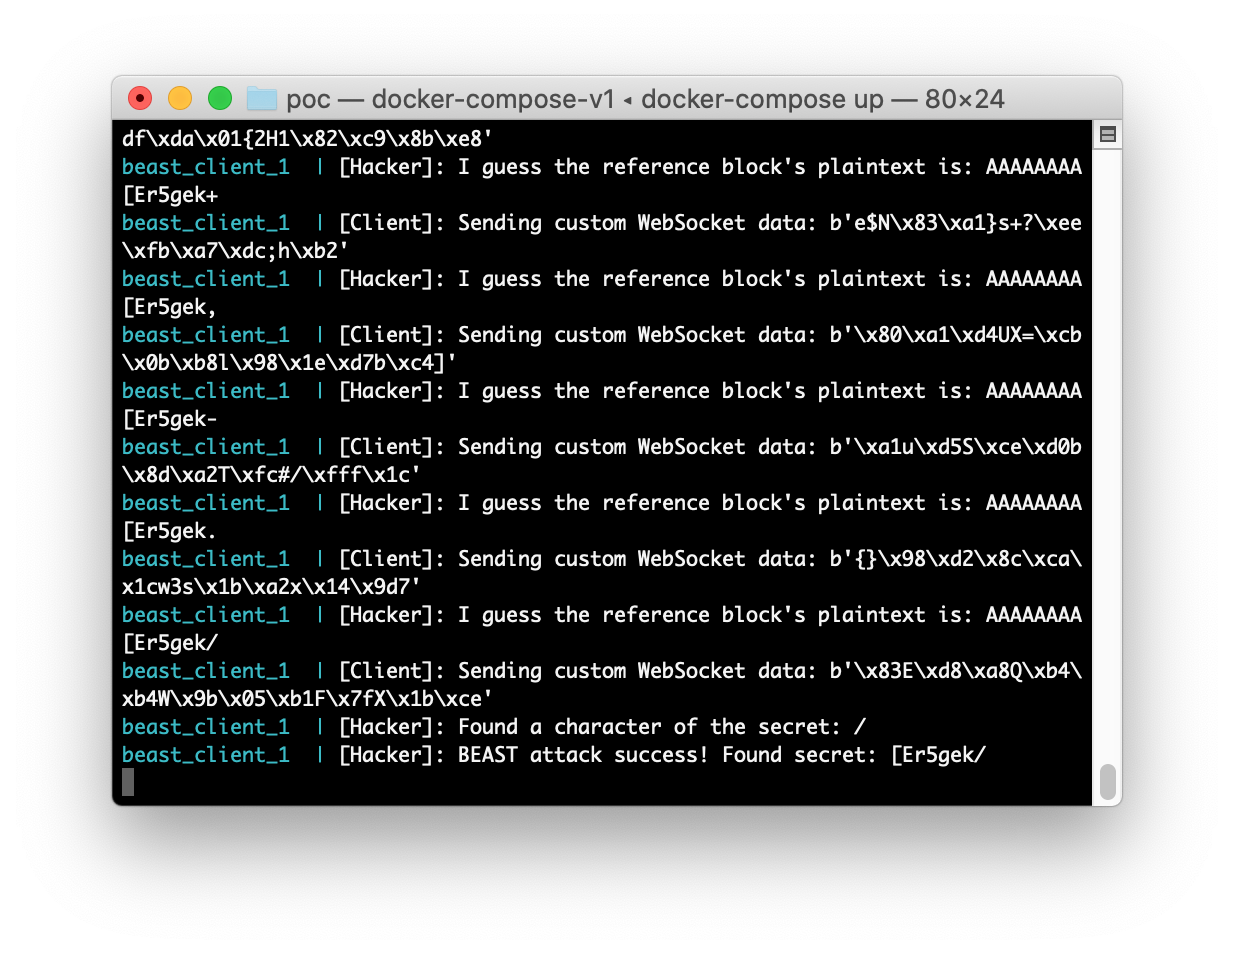
\includegraphics[keepaspectratio, width=\linewidth]{./figures/simulation.png}
    \caption{result of the simulation}
    \label{fig:simulation}
\end{figure}

\section{Feasibility and Defense}
\subsection{Feasibility}
While BEAST attacks are theoretically feasible, with the enhancement of security
features of browsers and other clients, BEAST attacks are less and less practical
for an attacker to exploit.

\subsubsection{Cross-Origin Resource Sharing (CORS)}
CORS is a group of policies to regulate the contents of cross-origin requests.
An attacker cannot make a request to other sites using JavaScript. If an attacker
wants to send some requests to Facebook, they will be rejected by browser's policies.

That is to say, when attackers want the clients to forge a request to websites with
credentials. These requests will not be sent. Thus, BEAST attacks will not work
any longer.

\subsubsection{WebSocket mask}
WebSocket is not subject to CORS policies, and it can be also wrapped by TLS.
It seems that WebSocket will be a good choice to implement BEAST attack.

However, in modern clients, WebSocket payloads are masked\cite{mask} by a value shown in \ref{fig:websocket-mask}.

\begin{figure}[htb]
    \centering
    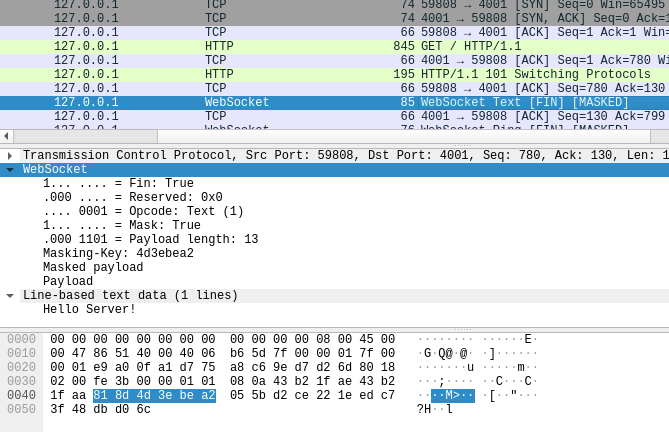
\includegraphics[keepaspectratio, width=\linewidth]{./figures/websocket-mask.png}
    \caption{WebSocket mask}
    \label{fig:websocket-mask}
\end{figure}

Besides, WebSocket prepends extra bits before the real payload. It is still hard to
control the block boundary.

The mask makes it hard for attackers to do BEAST attacks, since the attacker will not be able to
gain complete control over any plaintext block, thus losing the chosen plaintext privilege.

\subsection{Defense}
BEAST attacks make use of a flaw in the specification of TLS 1.0, and the attack only
works for block ciphers. That is to say, stream ciphers with TLS 1.0 are not
vulnerable to BEAST attacks.

However, TLS 1.0 is still vulnerable to other attacks when using stream ciphers (e.g. RC4).
Therefore, a much more direct way is just to abandon TLS 1.0, and update to later TLS
versions.

Many modern browsers and clients have also limited users to browse those sites
with TLS 1.0 enabled alone. This kind of action will boost organizations to update their
websites TLS versions. Today most popular sites on the internet have dropped support for TLS 1.0.

Yet for new services on the internet, it should be noticed that popular web servers such as Apache
and Nginx still supports TLS 1.0 by default\cite{disable} and should be manually disabled.

\section{Detection}
Detection of server vulnerability is easy. We only need to scan all cipher suites accepted by the TLS
1.0 server. This can be done with \textit{nmap}, with the following command:
\begin{lstlisting}
nmap --script \
ssl-enum-ciphers -p <PORT> <DOMAIN NAME>
\end{lstlisting}

Here we will propose a method to detect BEAST vulnerability of a server, together with a
Python script which displays clearly whether each cipher suite is vulnerable.

At the stage of TLS handshake, a cipher suite will be selected through these steps:

\begin{enumerate}
    \item (Client Hello) Client sent a list of accepted cipher suites.
    \item (Server Hello) Server chose a best accepted cipher suite, or a handshake failure occured.
\end{enumerate}

\begin{figure}[htb]
    \centering
    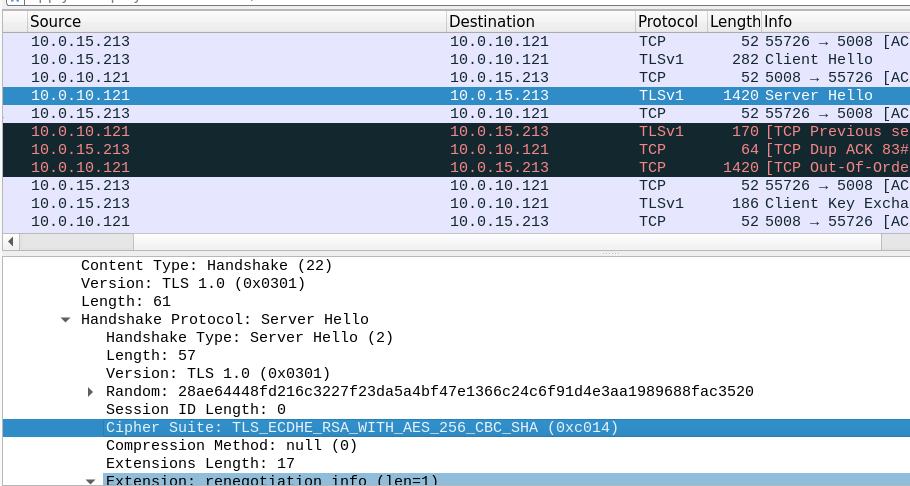
\includegraphics[keepaspectratio, width=\linewidth]{./figures/tls-handshake-cipher-spec.png}
    \caption{Negotiation on the cipher suite}
\end{figure}

Based on this, a scanner could change the list of cipher suites to enumerate all
cipher suites that the server will accept.

The server is vulnerable to BEAST attacks if it accepts TLS 1.0 handshake and support
cipher suites with CBC modes.

\begin{lstlisting}[language=bash]
python scan.py <HOST> <PORT>
\end{lstlisting}

The \texttt{openssl} utility is able to start a TLS server with many options.

\begin{lstlisting}
openssl s_server \
    -CAfile ca_cert.pem \
    -cert server_cert.pem \
    -key server_key.pem \
    -HTTP -port 5008 -tls1
\end{lstlisting}

\begin{figure}[htb]
    \centering
    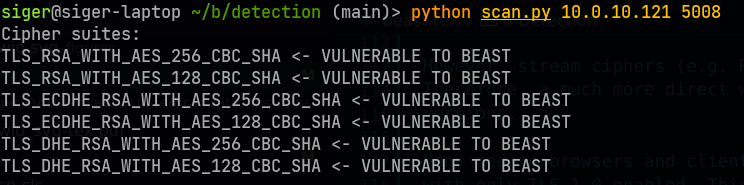
\includegraphics[keepaspectratio, width=\linewidth]{./figures/detection-output.png}
    \caption{Detection output on a TLS 1.0 server}
\end{figure}

% \subsection{}
%ACKNOWLEDGMENTS are optional
% The following two commands are all you need in the
% initial runs of your .tex file to
% produce the bibliography for the citations in your paper.
\bibliographystyle{abbrv}
\bibliography{beast}  % sigproc.bib is the name of the Bibliography in this case
% You must have a proper ".bib" file
%  and remember to run:
% latex bibtex latex latex
% to resolve all references
%
% ACM needs 'a single self-contained file'!
%
%APPENDICES are optional
\balancecolumns
\appendix
\section{Trials and errors in simulation}
In trying to recreate the BEAST attack, we first wanted to implement a full-fledged attack scenario
with a real vulnerable HTTPS server and a real browser client. The server part was easy. It only
required a specially configured Apache httpd server. Yet we ran into several issues when trying to
implement the attack, which forced us to abandon the original plan.
\subsection{Browsers mysteriously splitting requests}
We issued a normal request to the server using a common browser (Firefox) and used Wireshark to
sniff the packets and observe the packet structure. In the process, we noticed that Firefox
mysteriously split our very short request plaintext into two parts as in \ref{fig:split}:
one with a single 'G' as in the HTTP 'GET' verb, the other with the rest of the request.

\begin{figure}[htb]
    \centering
    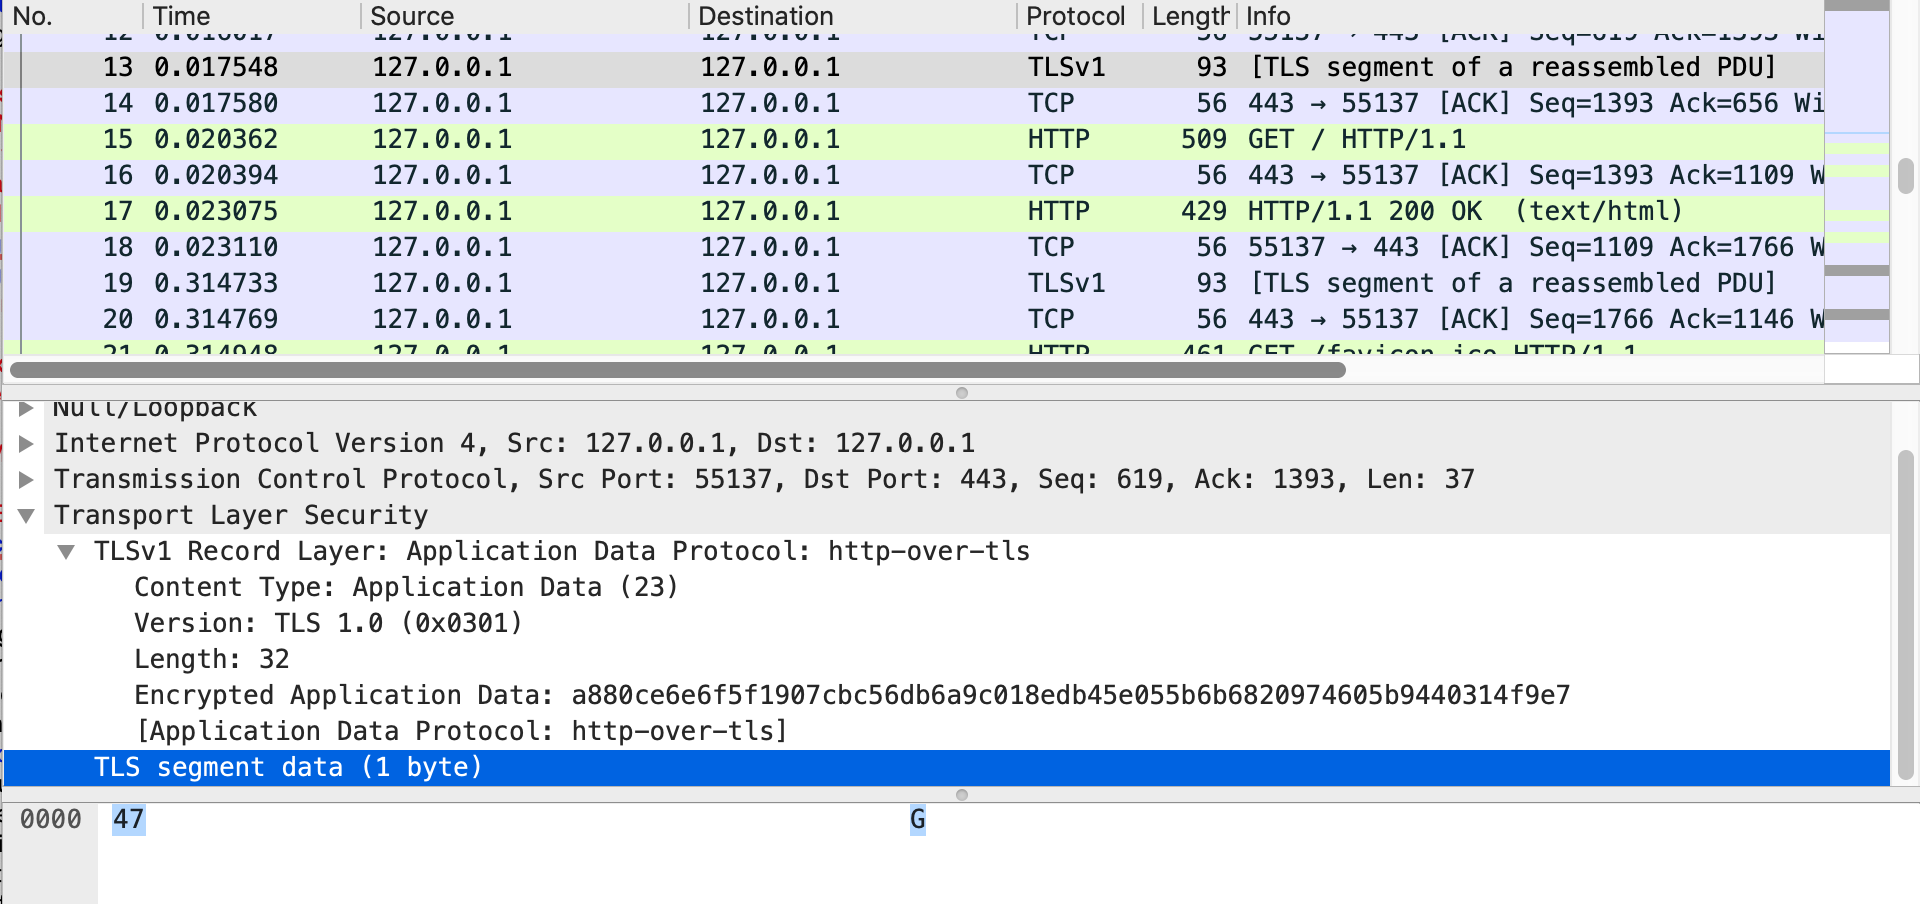
\includegraphics[keepaspectratio, width=\linewidth]{./figures/split.png}
    \caption{a TLS record with only 1 byte of plaintext}
    \label{fig:split}
\end{figure}
Notice that in this figure, the plaintext 'G' is padded to as long as 2 blocks (32 bytes) and the rest of
the request is found in packet No.15.
After several retries, we found that this behavior is consistent between requests in Firefox and it only
splits requests this way when using a TLS 1.0 protocol. Also, experiments conducted with \textit{curl}
shows that curl is not doing this. Although in this case chosen boundary privilege can still be
obtained, the attacker is now much harder to mount the attack without prior knowledge of the
browser's behavior. So splitting requests might also be a simple yet effective countermeasure
against the BEAST attack. Good job, Firefox developers!
\subsection{Masking is mandatory}
As we mentioned in Section 6.1.2, the use of WebSocket mask prevents the attacker from gaining
chosen plaintext privilege. The randomness and unpredictable nature of masks for each message
made it impossible for any client JavaScript to control the plaintext of a block. We looked for ways
to disable masking for our demonstration purpose, only to sadly realize that it is required, not
recommended by design\cite{rfc6455} that the client uses a mask when transmitting messages.
This is actually not to defend against BEAST attacks, but unfortunately it broke our original plan.

\section{Scanning the internet}
We scanned the 10 most visited websites in China using our detection tool and found that
(surprisingly) 7 out of 10 sites still supports at least one encryption scheme vulnerable to the BEAST
attack. The other 3 sites either do not support TLS 1.0 with CBC block ciphers or drop TLS 1.0
requests immediately.

We also did a scan on Prof.Anderson's site and it turned out that our professor did not give us the
chance to try out the attack on his site by not supporting TLS 1.0 entirely.


\balancecolumns
\end{document}
